\documentclass[aspectratio=169]{beamer}

% Theme
\usetheme{Madrid}
\usecolortheme{seahorse}
\setbeamertemplate{navigation symbols}{}
\setbeamertemplate{footline}[frame number]

% Encoding & fonts
\usepackage[T1]{fontenc}
\usepackage[utf8]{inputenc}

% Packages
\usepackage{amsmath,amssymb}
\usepackage{algorithm}      % keep available for later slides (avoid floats inside columns)
\usepackage{algpseudocode}
\usepackage{tikz}
\usetikzlibrary{calc}
\usetikzlibrary{arrows.meta,positioning,shapes.geometric}

% Colors
\definecolor{pivotblue}{RGB}{32,102,170}
\definecolor{updategreen}{RGB}{56,142,60}
\definecolor{depred}{RGB}{198,40,40}
\definecolor{accent}{RGB}{123,31,162}

% Compact bullets
\newenvironment{tightitem}{%
  \begin{itemize}\setlength{\itemsep}{2pt}\setlength{\parskip}{0pt}
}{\end{itemize}}

% Metadata
\title[Parallel In-place QR for SLSQP]{Efficient Task-Graph Scheduling for In-place Householder QR in SLSQP}
\subtitle{Dependency-aware two-queue scheduling for barrier-free parallelism}
\author{Your Name}
\institute{Your Lab / Department, Your Institute}
\date{Euro-Par 2025}

\begin{document}

\begin{frame}
  \titlepage
\end{frame}

% Import slides
% Slide 1 — Matrix QR Factorization (with flowchart)
\begin{frame}{Matrix QR Factorization}
  \begin{columns}[T,onlytextwidth]

    \column{0.56\textwidth}
    \begin{tightitem}
      \item \textbf{Goal:} Factor a full-rank $m\times n$ matrix $A$ as $A = Q\,R$
            with $Q^{\top}Q = I$ and $R$ upper triangular.
      \item \textbf{Why QR (vs.\ normal equations)?} Numerically stable:
            avoids forming $A^{\top}A$; solve least-squares via $R x = Q^{\top} b$.
      \item \textbf{Householder idea:} For each column, build a reflector that
            zeros subdiagonal entries; store $Q$ \emph{implicitly} via vectors $u$
            and scalars $b$.
      \item \textbf{In-place layout (used later by SLSQP):} keep $R$ in the
            upper triangle; store Householder vectors in the strict lower
            triangle and scalars $b[i]$ in a side array.
    \end{tightitem}

    \vspace{2mm}
    \small \textit{Next: the sequential algorithm and a diagram that mirrors its steps.}

    \column{0.44\textwidth}
    \centering
    % Compact flowchart (fits the column)
    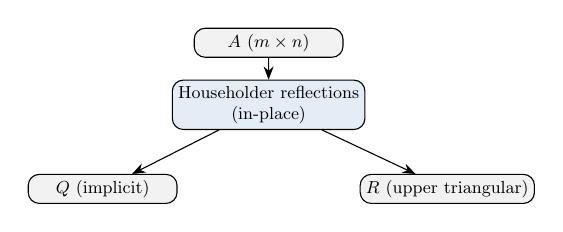
\begin{tikzpicture}[font=\small, node distance=4mm, every node/.style={transform shape}, scale=0.7]
      \tikzstyle{box}=[rectangle,rounded corners,draw,align=center,inner sep=3pt,minimum width=2.7cm,fill=gray!10]
      \node[box] (A) {$A$ ($m\times n$)};
      \node[box,fill=pivotblue!12,below=of A] (HH) {Householder reflections\\(in-place)};
      \node[box,below left=8mm and -1mm of HH] (Q) {$Q$ (implicit)};
      \node[box,below right=8mm and -1mm of HH] (R) {$R$ (upper triangular)};
      \draw[-{Stealth}] (A) -- (HH);
      \draw[-{Stealth}] (HH) -- (Q);
      \draw[-{Stealth}] (HH) -- (R);

    \end{tikzpicture}

  \end{columns}
\end{frame}

% Slide 2 — Householder QR — Sequential Algorithm (paper-style)
\begin{frame}{Householder QR — Sequential Algorithm}
  \begin{columns}[T,onlytextwidth]

    % ----- Left: Algorithm (paper-style names) -----
    \column{0.56\textwidth}
    \begin{block}{Sequential in-place Householder QR}
      \begin{algorithmic}[1]
        \State \textbf{Input:} $A\in\mathbb{R}^{m\times n}$
        \State \textbf{Output:} Upper $R$, reflectors in lower, scalars $b[1..\min(m,n)]$
        \For{$i=1$ to $\min(m,n)$}
          \State $(u,b)\leftarrow$ \textcolor{pivotblue}{\textsc{update\_pivot\_row}}$(A,i)$
          \For{$j=i+1$ to $n$}
            \State \textcolor{updategreen}{\textsc{update\_non\_pivot\_rows}}$(A,i,j,u,b)$
          \EndFor
        \EndFor
      \end{algorithmic}
    \end{block}

    % ----- Right: Flowchart that mirrors the algorithm (safe TikZ) -----
    \column{0.44\textwidth}
    \centering
    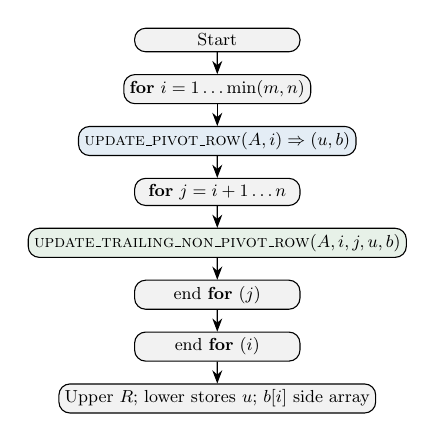
\begin{tikzpicture}[font=\small, node distance=4mm, every node/.style={transform shape}, scale=0.7]
      \tikzstyle{p}=[rectangle,rounded corners,draw,align=center,inner sep=3pt,minimum width=3.0cm,fill=gray!10]
      \tikzstyle{actA}=[p,fill=pivotblue!12]
      \tikzstyle{actB}=[p,fill=updategreen!12]

      % loop structure
      \node[p] (start) {Start};
      \node[p,below=of start] (loopi) {\textbf{for} $i=1\ldots \min(m,n)$};
      \node[actA,below=of loopi] (pivot) {\textsc{update\_pivot\_row}$(A,i)\Rightarrow (u,b)$};
      \node[p,below=of pivot] (loopj) {\textbf{for} $j=i+1\ldots n$};
      \node[actB,below=of loopj] (trail) {\textsc{update\_trailing\_non\_pivot\_row}$(A,i,j,u,b)$};
      \node[p,below=of trail] (endj) {end \textbf{for} ($j$)};
      \node[p,below=of endj] (endi) {end \textbf{for} ($i$)};
      \node[p,below=of endi] (done) {Upper $R$; lower stores $u$; $b[i]$ side array};

      % arrows
      \draw[-{Stealth}] (start) -- (loopi);
      \draw[-{Stealth}] (loopi) -- (pivot);
      \draw[-{Stealth}] (pivot) -- (loopj);
      \draw[-{Stealth}] (loopj) -- (trail);
      \draw[-{Stealth}] (trail) -- (endj);
      \draw[-{Stealth}] (endj) -- (endi);
      \draw[-{Stealth}] (endi) -- (done);
    \end{tikzpicture}

    \vspace{1mm}
    \small \textit{In-place contract: $R$ in upper triangle; reflectors $u$ in lower; scalars $b[i]$ are preserved for SLSQP.}

  \end{columns}
\end{frame}

% Slide 3 — Where QR Lives in SLSQP
\begin{frame}{Where QR Lives in SLSQP}
  \begin{columns}[T,onlytextwidth]

    % ---- Left: key points ----
    \column{0.55\textwidth}
    \begin{tightitem}
      \item SLSQP solves a sequence of quadratic subproblems with linearized constraints.
      \item Each iteration computes a descent direction from a KKT-like system.
      \item Implementation relies on \textbf{in-place Householder QR}:
            \begin{tightitem}
              \item keeps $R$ in the upper triangle,
              \item stores reflectors $u$ in the lower triangle,
              \item keeps scalars $b[i]$ alongside.
            \end{tightitem}
      \item \textbf{Why in-place matters here:} the intermediate reflectors
            \((u,b)\) are \emph{consumed immediately} in the SLSQP iteration,
            not just the final $(Q,R)$.
    \end{tightitem}

    % ---- Right: SLSQP pipeline diagram ----
    \column{0.45\textwidth}
    \centering
    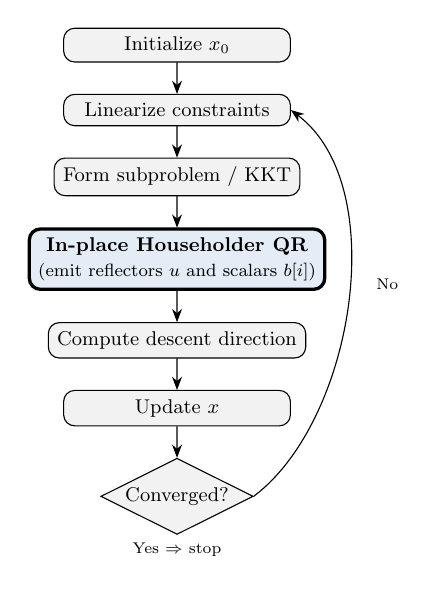
\begin{tikzpicture}[font=\small, node distance=5mm,
                        every node/.style={transform shape},
                        scale=0.8]
      % styles
      \tikzstyle{box}=[rectangle,rounded corners,draw,align=center,
                       inner sep=4pt,minimum width=3.6cm,fill=gray!10]
      \tikzstyle{qrbox}=[box,fill=pivotblue!12,very thick]
      \tikzstyle{cond}=[diamond,aspect=2,draw,align=center,inner sep=1pt,fill=gray!10]

      % nodes
      \node[box]   (init) {Initialize $x_0$};
      \node[box,below=of init] (lin)  {Linearize constraints};
      \node[box,below=of lin]  (kkt)  {Form subproblem / KKT};
      \node[qrbox,below=of kkt](qr)   {\textbf{In-place Householder QR}\\
                                       \footnotesize (emit reflectors $u$ and scalars $b[i]$)};
      \node[box,below=of qr]   (dir)  {Compute descent direction};
      \node[box,below=of dir]  (upd)  {Update $x$};
      \node[cond,below=of upd] (chk)  {Converged?};

      % arrows
      \draw[-{Stealth}] (init) -- (lin);
      \draw[-{Stealth}] (lin)  -- (kkt);
      \draw[-{Stealth}] (kkt)  -- (qr);
      \draw[-{Stealth}] (qr)   -- (dir);
      \draw[-{Stealth}] (dir)  -- (upd);
      \draw[-{Stealth}] (upd)  -- (chk);

      % loop-back arrow
      \draw[-{Stealth}] (chk.east) .. controls +(1.6,1.2) and +(1.6,-1.2) .. (lin.east);

      % yes/no labels (small)
      \node[anchor=west] at ($(chk.east)!0.55!(lin.east)+(1.5,0.0)$) {\scriptsize No};
      \node[anchor=north] at (chk.south) {\scriptsize Yes $\Rightarrow$ stop};
    \end{tikzpicture}


  \end{columns}
\end{frame}

% Slide 4 — QR as a Task DAG (Problem Statement, with paper figure replicated in TikZ)
\begin{frame}{QR as a Task DAG — Problem Statement}
\small
\begin{columns}[T,onlytextwidth]

  % ---------- LEFT: context & problem ----------
  \column{0.52\textwidth}
  \begin{block}{Tasks and what they represent}
    \begin{tightitem}
      \item In-place Householder QR is modeled as tasks $T_{i,j}$ over the upper triangle ($1\!\le\!i\!\le\!j\!\le\!n$).

      \item $\mathrm{parents}(T_{i,j})=\{\,T_{i,i}\text{ (pivot)},\;T_{i-1,j}\text{ (prev.\ row)}\,\}$ .
      \item The diagonal $\{T_{1,1},T_{2,2},\ldots\}$ is the \textbf{critical path}; finishing it unlocks width.
      \item A task is \emph{ready} to be executed once all its parents complete execution.
    \end{tightitem}
  \end{block}

  \vspace{0.5mm}
  \begin{block}{Scheduling goal}
    \begin{tightitem}
      \item Execute this DAG on $p$ threads \textbf{without global barriers}, keeping workers on \emph{ready} tasks and releasing the critical path early—while preserving the in-place interface SLSQP needs.
    \end{tightitem}
  \end{block}

    % ---- Right: TaskGraph figure (ported from paper’s TikZ) ----
    \column{0.50\textwidth}
    \centering
    % color from the paper
    \definecolor{lightblue}{RGB}{173,216,230}
    \begin{tikzpicture}[node distance=1cm and 0.5cm, scale=0.55, transform shape]
      % Nodes - Row 1
      \node[draw, circle, fill=lightblue] (T11) at (0,0) {$T_{1,1}$};
      \node[draw, circle, fill=lightblue] (T12) at (1.4,-1.2) {$T_{1,2}$};
      \node[draw, circle] (T13) at (2.6,-1.2) {$T_{1,3}$};
      \node[draw, circle] (T14) at (3.8,-1.2) {$T_{1,4}$};
      \node[draw, circle] (T15) at (4.9,-1.2) {$T_{1,5}$};

      % Nodes - Row 2
      \node[draw, circle, fill=lightblue] (T22) at (1.4,-2.5) {$T_{2,2}$};
      \node[draw, circle, fill=lightblue] (T23) at (2.6,-3.5) {$T_{2,3}$};
      \node[draw, circle] (T24) at (3.8,-3.5) {$T_{2,4}$};
      \node[draw, circle] (T25) at (4.9,-3.5) {$T_{2,5}$};

      % Nodes - Row 3
      \node[draw, circle, fill=lightblue] (T33) at (2.6,-4.8) {$T_{3,3}$};
      \node[draw, circle, fill=lightblue] (T34) at (3.8,-5.8) {$T_{3,4}$};
      \node[draw, circle] (T35) at (4.9,-5.8) {$T_{3,5}$};

      % Nodes - Row 4
      \node[draw, circle, fill=lightblue] (T44) at (3.8,-7.1) {$T_{4,4}$};
      \node[draw, circle, fill=lightblue] (T45) at (4.9,-8.1) {$T_{4,5}$};

      % Nodes - Row 5
      \node[draw, circle, fill=lightblue] (T55) at (4.9,-9.7) {$T_{5,5}$};

      % Edges (ported from paper)
      \draw[->] (T11) -- (T12);
      \draw[->] (T12) -- (T22);
      \draw[->] (T13) -- (T23);
      \draw[->] (T14) -- (T24);
      \draw[->] (T15) -- (T25);
      \draw[->, bend left] (T11) to (T13);
      \draw[->, bend left] (T11) to (T14);
      \draw[->, bend left] (T11) to (T15);

      \draw[->] (T22) -- (T23);
      \draw[->] (T24) -- (T34);
      \draw[->] (T25) -- (T35);
      \draw[->, bend left] (T22) to (T24);
      \draw[->, bend left] (T22) to (T25);

      \draw[->] (T23) -- (T33);
      \draw[->, bend left] (T33) to (T34);
      \draw[->, bend left] (T33) to (T35);

      \draw[->] (T34) -- (T44);
      \draw[->] (T35) -- (T45);
      \draw[->, bend left] (T44) to (T45);

      \draw[->] (T45) -- (T55);
    \end{tikzpicture}

    \vspace{1mm}
    {\scriptsize \emph{“TaskGraph for Triangular System”}}

  \end{columns}
\end{frame}

% Slide 5 — Barrier Scheduling on the QR DAG (Baseline)
\begin{frame}{Barrier Scheduling on the QR DAG (Baseline)}
% --- FONT SIZE DECREASED FROM \small TO \footnotesize ---
\footnotesize
\begin{columns}[T,onlytextwidth]

  % ---------- LEFT ----------
  \column{0.35\textwidth}

  \begin{block}{Mechanics (per iteration $i$)}
    \begin{tightitem}
      \item \textbf{Phase A:} compute pivot task $T_{i,i}$ to form $(u_i,b_i)$ and write $R/u$ in-place.
      \item \textbf{Barrier 1:} ensure all workers see $(u_i,b_i)$.
      \item \textbf{Phase B:} apply $(u_i,b_i)$ to updates $T_{i,j}$ for all $j>i$.
      \item \textbf{Barrier 2:} finalize iteration $i$ before entering $i{+}1$.
    \end{tightitem}
  \end{block}

  % ---------- RIGHT ----------
  \column{0.60\textwidth}
    \begin{block}{What this preserves}
    \begin{tightitem}
      \item Dependency rule: $\mathrm{parents}(T_{i,j})=\{\,T_{i,i},\,T_{i-1,j}\,\}$ \;(ignore $T_{0,j}$).
      \item In-place contract for SLSQP: upper $\rightarrow R$, lower $\rightarrow u$, side array $\rightarrow b[i]$.
    \end{tightitem}
  \end{block}

\centering
  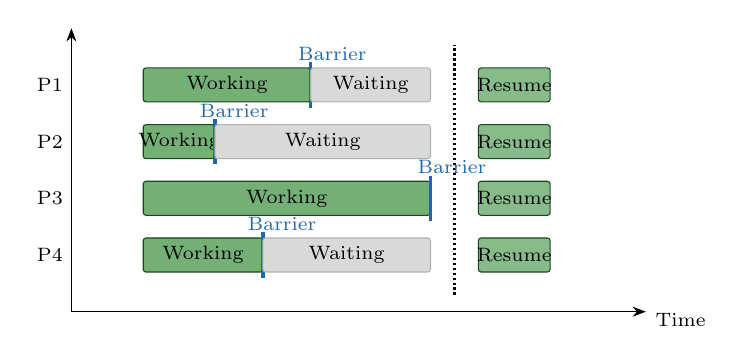
\begin{tikzpicture}[x=0.38cm,y=0.9cm,>=Stealth, every node/.style={font=\scriptsize}, scale=0.80 ]
    % Styles
    \tikzset{work/.style   ={fill=updategreen!70,draw=updategreen!50!black,rounded corners=1pt}}
    \tikzset{wait/.style   ={fill=gray!30,      draw=gray!60,            rounded corners=1pt}}
    \tikzset{resume/.style ={fill=updategreen!60,draw=updategreen!50!black,rounded corners=1pt}}
    \tikzset{barline/.style={draw=pivotblue,very thick}}
    \tikzset{bartext/.style={fill=none,text=pivotblue}}

    % Axes
    \draw[->] (0,0) -- (24,0);
    \draw[->] (0,0) -- (0,5);
    \node[anchor=west] at (24,-0.15) {Time};

    % Lane labels
    \node at (-0.9,4) {P1};
    \node at (-0.9,3) {P2};
    \node at (-0.9,2) {P3};
    \node at (-0.9,1) {P4};

    % Global (iteration) barrier (dotted vertical guide)
    \draw[densely dotted,thick] (16,0.3) -- (16,4.7);

    % P1 timeline
    \draw[work]   (3,3.7) rectangle node{Working} (10,4.3);
    \draw[barline](10,3.6) -- (10,4.4);  \node[bartext] at (10.9,4.55) {Barrier};
    \draw[wait]   (10,3.7) rectangle node{Waiting} (15,4.3);
    \draw[resume] (17,3.7) rectangle node{Resume}  (20,4.3);

    % P2 timeline
    \draw[work]   (3,2.7) rectangle node{Working} (6,3.3);
    \draw[barline](6,2.6) -- (6,3.4);   \node[bartext] at (6.8,3.55) {Barrier};
    \draw[wait]   (6,2.7) rectangle node{Waiting} (15,3.3);
    \draw[resume] (17,2.7) rectangle node{Resume}  (20,3.3);

    % P3 timeline
    \draw[work]   (3,1.7) rectangle node{Working} (15,2.3);
    \draw[barline](15,1.6) -- (15,2.4); \node[bartext] at (15.9,2.55) {Barrier};
    \draw[resume] (17,1.7) rectangle node{Resume}  (20,2.3);

    % P4 timeline
    \draw[work]   (3,0.7) rectangle node{Working} (8,1.3);
    \draw[barline](8,0.6) -- (8,1.4);   \node[bartext] at (8.8,1.55) {Barrier};
    \draw[wait]   (8,0.7) rectangle node{Waiting} (15,1.3);
    \draw[resume] (17,0.7) rectangle node{Resume}  (20,1.3);
  \end{tikzpicture}

  % --- FONT SIZE OF CAPTION DECREASED ---
  {\scriptsize Fast threads wait at the barrier; useful overlap is lost until all reach the sync point.}
\end{columns}
\end{frame}
% Slide 6 — Two-Queue Scheduler: Concept (enqueue-to-main, move-to-wait-on-check)
\begin{frame}{Two-Queue Scheduler — Concept}
\small
\begin{columns}[T,onlytextwidth]
  \column{0.38\textwidth}
  \begin{block}{Queues (by design)}
    \begin{tightitem}
      \item \textbf{Main queue (ready-first policy):} all newly spawned tasks are enqueued here.
      \item \textbf{Wait queue:} holds tasks that were \emph{dequeued} from main but failed the readiness check
            (e.g., missing $T_{i-1,j}$).
      \item Workers pop from \emph{main}; after executing a task, each child is enqueued to \emph{main}.
      \item A promotion step scans \emph{wait} and moves newly-ready tasks back to \emph{main}. No global barriers.
    \end{tightitem}
  \end{block}

  \column{0.60\textwidth}
  \centering
  \begin{tikzpicture}[x=0.45cm,y=0.45cm,>=Stealth, every node/.style={transform shape,font=\scriptsize}]
    \tikzset{queue/.style={draw,rounded corners=0pt}}
    \tikzset{slot/.style ={draw,gray!70}}
    \tikzset{qlabel/.style={draw,white,fill=white,inner sep=2pt}}
    \tikzset{anno/.style ={align=left}}

    % Top (Main)
    \draw[queue,gray!70] (0,10) -- (18,10);
    \draw[queue,gray!70] (0,8.7) -- (18,8.7);
    \foreach \x in {5,9.5,14}{ \draw[slot] (\x,8.7) -- (\x,10); }
    \node[qlabel,anchor=east] at (17.5,9.35) {Main Queue};

    % Arrow: tasks enter main
    \draw[-{Stealth},thick] (-6,9.35) -- (-0.2,9.35);
    \node[anno,anchor=west] at (-6,10.0) {Tasks are\\enqueued into\\the main queue};

    % Middle arrows (check may send to wait; promotion returns to main)
    \draw[-{Stealth},gray!70,thick] (8.8,8.3) -- (8.8,5.0);  % to wait on failed check
    \draw[-{Stealth},gray!70,thick] (13.6,5.0) -- (13.6,8.3); % promotion back

    % Bottom (Wait)
    \draw[queue,gray!70] (0,3.7) -- (18,3.7);
    \draw[queue,gray!70] (0,2.4) -- (18,2.4);
    \foreach \x in {5,9.5,14}{ \draw[slot] (\x,2.4) -- (\x,3.7); }
    \node[qlabel,anchor=east] at (17.5,3.05) {Wait Queue};
  \end{tikzpicture}
\end{columns}
\end{frame}

% Slide 7 — Two-Queue Scheduler: Demo (A — start)
\begin{frame}{Two-Queue Scheduler — Demo (A: Start)}
\small
\begin{columns}[T,onlytextwidth]
  \column{0.46\textwidth}
  \begin{block}{State A}
    \begin{tightitem}
      \item Parents$(T_{i,j})=\{\,T_{i,i},\,T_{i-1,j}\,\}$; ignore $T_{0,j}$.
      \item Initially only the pivot $T_{1,1}$ is ready $\Rightarrow$ in \textbf{main}.
      \item \textbf{Wait is empty.} Nothing goes to wait until a dequeued task fails its check.
    \end{tightitem}
  \end{block}

  \column{0.54\textwidth}
  \centering
  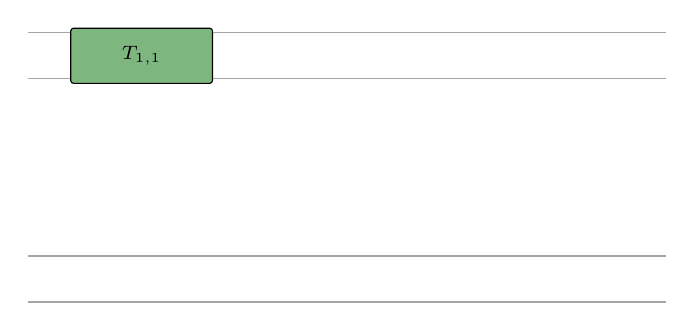
\begin{tikzpicture}[x=0.45cm,y=0.45cm,>=Stealth, every node/.style={transform shape,font=\scriptsize}]
    \tikzset{queue/.style={draw,rounded corners=0pt}}
    \tikzset{ready/.style={draw,fill=updategreen!65,rounded corners=1pt}}
    \tikzset{waitt/.style={draw,fill=gray!25,rounded corners=1pt}}
    \tikzset{qlabel/.style={draw,white,fill=white,inner sep=2pt}}

    % Main
    \draw[queue,gray!70] (0,10) -- (18,10);
    \draw[queue,gray!70] (0,8.7) -- (18,8.7);
    \node[qlabel,anchor=east] at (17.5,9.35) {Main Queue};
    \node[ready,minimum width=1.8cm,minimum height=0.7cm] at (3.2,9.35) {$T_{1,1}$};

    % Wait (empty)
    \draw[queue,gray!70] (0,3.7) -- (18,3.7);
    \draw[queue,gray!70] (0,2.4) -- (18,2.4);
    \node[qlabel,anchor=east] at (17.5,3.05) {Wait Queue};
  \end{tikzpicture}
\end{columns}
\end{frame}

% Slide 8 — Two-Queue Scheduler: Demo (B — after T11 finishes)
\begin{frame}{Two-Queue Scheduler — Demo (B: After $T_{1,1}$)}
\small
\begin{columns}[T,onlytextwidth]
  \column{0.46\textwidth}
  \begin{block}{State B}
    \begin{tightitem}
      \item Executed $T_{1,1}$; it enqueues its children $T_{1,j}$ ($j>1$) to \textbf{main}.
      \item Workers pop from \textbf{main} and execute $T_{1,2},T_{1,3},\ldots$
      \item \textbf{Wait is still empty.}
    \end{tightitem}
  \end{block}

  \column{0.54\textwidth}
  \centering
  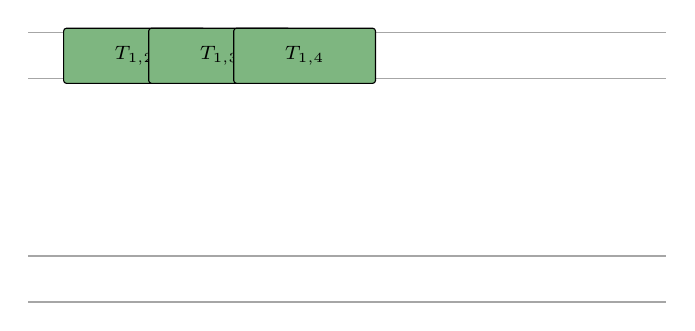
\begin{tikzpicture}[x=0.45cm,y=0.45cm,>=Stealth, every node/.style={transform shape,font=\scriptsize}]
    \tikzset{queue/.style={draw,rounded corners=0pt}}
    \tikzset{ready/.style={draw,fill=updategreen!65,rounded corners=1pt}}
    \tikzset{waitt/.style={draw,fill=gray!25,rounded corners=1pt}}
    \tikzset{qlabel/.style={draw,white,fill=white,inner sep=2pt}}

    % Main
    \draw[queue,gray!70] (0,10) -- (18,10);
    \draw[queue,gray!70] (0,8.7) -- (18,8.7);
    \node[qlabel,anchor=east] at (17.5,9.35) {Main Queue};
    \node[ready,minimum width=1.8cm,minimum height=0.7cm] at (3.0,9.35) {$T_{1,2}$};
    \node[ready,minimum width=1.8cm,minimum height=0.7cm] at (5.4,9.35) {$T_{1,3}$};
    \node[ready,minimum width=1.8cm,minimum height=0.7cm] at (7.8,9.35) {$T_{1,4}$};

    % Wait (empty)
    \draw[queue,gray!70] (0,3.7) -- (18,3.7);
    \draw[queue,gray!70] (0,2.4) -- (18,2.4);
    \node[qlabel,anchor=east] at (17.5,3.05) {Wait Queue};
  \end{tikzpicture}
\end{columns}
\end{frame}

% Slide 9 — Two-Queue Scheduler: Demo (C — dequeue check -> wait)
\begin{frame}{Two-Queue Scheduler — Demo (C: Dequeued \& Not Ready $\Rightarrow$ Wait)}
\small
\begin{columns}[T,onlytextwidth]
  \column{0.46\textwidth}
  \begin{block}{State C}
    \begin{tightitem}
      \item $T_{1,3}$ finishes and enqueues $T_{2,3}$ to \textbf{main}.
      \item A worker dequeues $T_{2,3}$ but its parent $T_{2,2}$ is not done yet.
      \item \textbf{Policy:} pushed to \textbf{wait} (will be promoted later).
    \end{tightitem}
  \end{block}

  \column{0.54\textwidth}
  \centering
  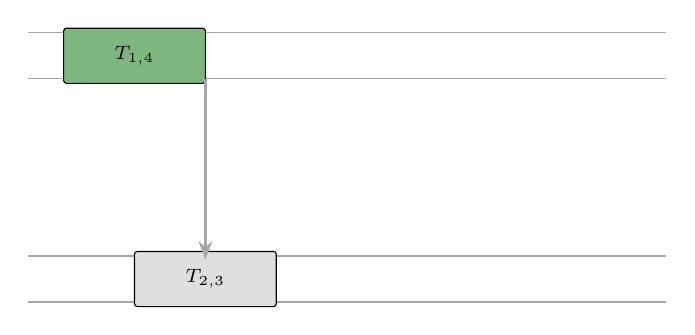
\begin{tikzpicture}[x=0.45cm,y=0.45cm,>=Stealth, every node/.style={transform shape,font=\scriptsize}]
    \tikzset{queue/.style={draw,rounded corners=0pt}}
    \tikzset{ready/.style={draw,fill=updategreen!65,rounded corners=1pt}}
    \tikzset{waitt/.style={draw,fill=gray!25,rounded corners=1pt}}
    \tikzset{qlabel/.style={draw,white,fill=white,inner sep=2pt}}

    % Main (T14 still there; T23 was popped and moved)
    \draw[queue,gray!70] (0,10) -- (18,10);
    \draw[queue,gray!70] (0,8.7) -- (18,8.7);
    \node[qlabel,anchor=east] at (17.5,9.35) {Main Queue};
    \node[ready,minimum width=1.8cm,minimum height=0.7cm] at (3.0,9.35) {$T_{1,4}$};

    % Wait (now holds T23)
    \draw[queue,gray!70] (0,3.7) -- (18,3.7);
    \draw[queue,gray!70] (0,2.4) -- (18,2.4);
    \node[qlabel,anchor=east] at (17.5,3.05) {Wait Queue};
    \node[waitt,minimum width=1.8cm,minimum height=0.7cm] at (5.0,3.05) {$T_{2,3}$};

    % Arrow showing move main -> wait
    \draw[-{Stealth},gray!70,thick] (5.0,8.7) -- (5.0,3.6);
  \end{tikzpicture}
\end{columns}
\end{frame}

\input{SLide10}
% Slide 11 — Two-Queue Scheduler: Flowchart (from source) + Pseudocode (smaller)
\begin{frame}{Two-Queue Scheduler — Flow \& Pseudocode}
\footnotesize
\begin{columns}[T,onlytextwidth]

  % -------- LEFT: pseudocode (compact) --------
  \column{0.50\textwidth}
\begin{block}{Pseudocode (ready-first, no global barriers)}
  % --- FONT SIZE DECREASED TO MAKE BLOCK MORE COMPACT ---
  \footnotesize
  \begin{algorithmic}[1]
    \State \textbf{Queues:} main (ready-first), wait
    \While{true}
      \State $t \gets$ pop(main)
      \If{$t = \varnothing$}
        \State promote\_ready(wait $\rightarrow$ main)
        \If{empty(main) \textbf{and} empty(wait)} \textbf{break} \EndIf
        \State \textbf{continue}
      \EndIf
      \If{\textbf{not} parents\_done($t$)} \Comment{e.g., missing $T_{i-1,j}$}
        \State push(wait, $t$) \Comment{dequeued but not ready}
        \State \textbf{continue}
      \EndIf
      \State execute($t$)
      \ForAll{$c \in$ children($t$)}
        \State push(main, $c$) \Comment{spawn to main (ready-first)}
      \EndFor
    \EndWhile
  \end{algorithmic}
\end{block}

  \vspace{1mm}
  \begin{block}{Readiness for $T_{i,j}$}
    parents\_done$(T_{i,j}) \iff T_{i,i}$ and $T_{i-1,j}$ complete \;(ignore $T_{0,j}$).
  \end{block}

  % -------- RIGHT: flowchart (ripped from your source, scaled down) --------
  \column{0.50\textwidth}
  % Styles as in methodology.tex
  \tikzstyle{startstop} = [rectangle, rounded corners, minimum width=2.2cm, minimum height=0.8cm, text centered, draw=black]
  \tikzstyle{process}   = [rectangle, minimum width=2.2cm, minimum height=0.8cm, text centered, draw=black]
  \tikzstyle{decision}  = [diamond,   minimum width=2.2cm, minimum height=0.7cm, text centered, draw=black, aspect=2]
  \tikzstyle{arrow}     = [thick,->,>=stealth]

  \centering
  \begin{tikzpicture}[node distance=1.3cm, scale=0.58, transform shape]
    % Nodes (as in your methodology.tex)
    \node (root)      [startstop, fill=red!30]                 {Root Node};
    \node (mq)        [process,   below of=root, fill=blue!30] {Main Queue};
    \node (executor)  [process,   below of=mq,   fill=green!30]{Executor};
    \node (dep)       [decision,  right of=executor, xshift=2.6cm, fill=yellow!30] {Dep Satisfied?};
    \node (wq)        [process,   below of=dep, yshift=-1.6cm,  fill=purple!30] {Wait Queue};
    \node (terminate) [startstop, below of=executor, yshift=-1.6cm, fill=orange!30] {Terminate};

    % Arrows (ported; two long paths reconstructed where upload was truncated)
    \draw [arrow] (root) -- node[right] {Enqueue} (mq);
    \draw [arrow] (mq) -- node[right] {Dequeue} (executor);
    \draw [arrow] (executor.east) -- node[above] {If children} (dep.west);
    \draw [arrow] (executor.south) -- node[right] {If no children} (terminate.north);

    % "No" path: dep -> wait queue (exact from source form)
    \draw [arrow] (dep.east) -- node[above] {No} ++(0.5,0)
                  -- node[midway,left] {Enqueue} ++(0,-3.0) -- (wq.east);

    % Return from wait queue to dep (reconstructed per source intent)
    \draw [arrow] (wq.west) -- ++(-0.5,0) -- ++(-0.3,0)
                  -- node[midway,right] {Dequeue} ++(0,1.6) -- ++(2.1,0) -- (dep.south);

    % "Yes" path: dep -> main queue (ported; label retained)
    \draw [arrow] (dep.north) |- node[right] {Yes} (mq.east);

  \end{tikzpicture}

\end{columns}
\end{frame}

% Slide 12 — Task Granularity: α (pivots) and β (rows)
\begin{frame}{Task Granularity — $\alpha$ (Pivots) and $\beta$ (Rows)}
\small
\begin{columns}[T,onlytextwidth]

  % ---------- LEFT: definitions & tradeoffs ----------
  \column{0.52\textwidth}
  \begin{block}{Definitions}
    \begin{tightitem}
      \item $\alpha$: number of \emph{pivot iterations} coalesced into one Task\,1 (build $\alpha$ reflectors).
      \item $\beta$: number of \emph{rows updated per task} in Task\,2 when applying a reflector.
      \item Spawn policy with two queues: children from any executed task $\rightarrow$ \textbf{main}; dequeued \& not-ready $\rightarrow$ \textbf{wait}.
    \end{tightitem}
  \end{block}

  \vspace{1mm}
  \begin{block}{Why these matter}
    \begin{tightitem}
      \item Small $\alpha,\beta$ $\Rightarrow$ many tiny tasks $\Rightarrow$ higher scheduling overhead.
      \item Large $\alpha$ $\Rightarrow$ fewer pivots in flight; risks underutilization if a pivot lags.
      \item Large $\beta$ $\Rightarrow$ less parallel width on updates; may help cache locality.
      \item Practical aim: balance \textbf{ready width} for the main queue vs.\ overhead and locality.
    \end{tightitem}
  \end{block}

  \vspace{1mm}
  {\scriptsize \emph{Note: we omit brute-force parameter sweeps here per talk guidelines.}}

  % ---------- RIGHT: visual (α block of pivots + β-row chunk updates) ----------
  \column{0.48\textwidth}
  \centering
  \begin{tikzpicture}[scale=0.78, every node/.style={transform shape,font=\scriptsize}]
    % Colors (use deck colors)
    \tikzset{pivotblk/.style ={fill=accent!20, draw=accent}}
    \tikzset{updateblk/.style={fill=updategreen!55, draw=updategreen!50!black}}
    \tikzset{outline/.style ={draw=gray!60}}

    % --- Upper-triangular grid (schematic) ---
    \def\n{7}
    \foreach \row in {1,...,\n}{
      \foreach \col in {\row,...,\n}{
        \node[outline,minimum width=0.42cm,minimum height=0.42cm] (A\row\col) at (0.42*\col,-0.42*\row) {};
      }
    }

    % --- Alpha window along the diagonal (α pivots coalesced) ---
    \def\alpha{3}
    \foreach \k in {1,...,\alpha}{
      \fill[pivotblk] (A\k\k.south west) rectangle (A\k\k.north east);
    }
    \node[anchor=west] at (0.42*(\alpha+1)+0.25,-0.42*1) {$\alpha$ pivots};

    % Arrows indicating children spawn to main (ready-first)
    \foreach \col in {2,...,\n}{
      \draw[-{Stealth[length=2mm]},accent] (A1 1.east) -- ++(0.22,0) |- (A1\col.center);
    }

    % --- Beta chunk on an update (rows-per-task) ---
    % choose reflector from i=2 applied to j=5; highlight beta rows
    \def\i{2} \def\j{5} \def\beta{2}
    % draw a bracket-like rectangle covering beta rows under column j
    \draw[updateblk,very thick,rounded corners]
      ($(A\i\j.south west)+(0.02,-0.02)$) rectangle
      ($(A\the\numexpr\i+\beta-1\relax\j.north east)+(-0.02,0.02)$);
    \node[anchor=west] at (0.42*(\j+1)+0.25,-0.42*(\i+\beta-0.5))
      {$\beta$ rows per update-task};

    % Tiny legend
    \draw[pivotblk] (0.3,-0.42*(\n+1)) rectangle ++(0.36,0.22);
    \node[anchor=west] at (0.7,-0.42*(\n+1)+0.11) {pivot block ($\alpha$)};
    \draw[updateblk,very thick] (2.4,-0.42*(\n+1)) rectangle ++(0.36,0.22);
    \node[anchor=west] at (2.8,-0.42*(\n+1)+0.11) {update chunk ($\beta$)};
  \end{tikzpicture}

\end{columns}
\end{frame}

\begin{frame}{Scalability with Matrix Size (26 \& 52 Threads)}
\small
\begin{columns}[T,onlytextwidth]
  \column{0.5\textwidth}
  \begin{block}{26 threads}
    % OPTION A (preferred): input the original TikZ/PGFPlots figure file from your source
    % \input{<PATH-TO-YOUR-SOURCE-FIGURE-FOR-4a>.tex}

    % OPTION B: include the compiled figure PDF/PNG from your source
    \centering
    \includegraphics[width=\linewidth]{figs/fig4a_exec_time_vs_size_26threads}%
  \end{block}

  \column{0.5\textwidth}
  \begin{block}{52 threads}
    % OPTION A
    % \input{<PATH-TO-YOUR-SOURCE-FIGURE-FOR-4b>.tex}

    % OPTION B
    \centering
    \includegraphics[width=\linewidth]{figs/fig4b_exec_time_vs_size_52threads}%
  \end{block}
\end{columns}

\vspace{1mm}
{\scriptsize Source: EuroPar camera-ready, Fig. 4a–b (exec. time vs matrix size).  :contentReference[oaicite:0]{index=0}  :contentReference[oaicite:1]{index=1} }
\end{frame}

\begin{frame}{Scalability with Threads (Throughput on Fixed Size)}
\small
% OPTION A (preferred): input the original TikZ/PGFPlots figure file from your source
% \input{<PATH-TO-YOUR-SOURCE-FIGURE-FOR-5>.tex}

% OPTION B: include the compiled figure PDF/PNG from your source


\vspace{1mm}
{\scriptsize Source: EuroPar camera-ready, Fig. 5 (Throughput evaluation).  :contentReference[oaicite:2]{index=2}  :contentReference[oaicite:3]{index=3} }
\end{frame}

\begin{frame}{Impact in SLSQP (End-to-End)}
\small
\begin{columns}[T,onlytextwidth]
  \column{0.58\textwidth}
  % OPTION A (preferred): input the original TikZ/PGFPlots figure file from your source
  % \input{<PATH-TO-YOUR-SOURCE-FIGURE-FOR-6>.tex}

  % OPTION B: include the compiled figure PDF/PNG from your source
  \centering
  \includegraphics[width=\linewidth]{figs/fig6_slsqp_performance}

  \vspace{1mm}
  {\scriptsize Source: EuroPar camera-ready, Fig. 6 (SLSQP performance).  :contentReference[oaicite:4]{index=4}  :contentReference[oaicite:5]{index=5} }

  \column{0.42\textwidth}
  \begin{block}{Key takeaway (from paper)}
    \begin{itemize}\itemsep3pt
      \item Parallel-QR SLSQP cuts wall-time dramatically as DOF grows.
      \item At DOF \(=2816\): \(\sim\)1.21 hrs (parallel QR) vs \(\sim\)18.91 hrs (sequential QR).%
      {\scriptsize \;:contentReference[oaicite:6]{index=6}}
    \end{itemize}
  \end{block}
\end{columns}
\end{frame}

% Slide 16 — Conclusion (+ Artifact QR)
% Tip: set your artifact URL here (repo or landing page)
\providecommand{\artifactURL}{https://example.com/your-artifact} % <-- replace

\begin{frame}{Conclusion \& Artifact}
\small
\begin{columns}[T,onlytextwidth]

  % -------- Left: concise conclusion --------
  \column{0.62\textwidth}
  \begin{block}{What we did}
    \begin{tightitem}
      \item Cast in-place Householder QR as a dependency DAG $T_{i,j}$ with parents $\{T_{i,i},\,T_{i-1,j}\}$.
      \item Replaced \textbf{global barriers} with a \textbf{two-queue, ready-first} scheduler:
            spawn $\rightarrow$ \emph{main}, dequeue-not-ready $\rightarrow$ \emph{wait}, then promote.
      \item Preserved SLSQP’s \emph{in-place} layout (upper $\rightarrow R$, lower $\rightarrow u$, side array $\rightarrow b$).
    \end{tightitem}
  \end{block}

  \vspace{1mm}
  \begin{block}{Why it works}
    \begin{tightitem}
      \item Reduces tail waiting; enables overlap once parents are satisfied.
      \item Keeps workers busy while releasing the \textbf{critical path} early.
      \item Plays well with task granularity ($\alpha$ pivots, $\beta$ rows).
    \end{tightitem}
  \end{block}

  \vspace{1mm}
  \begin{block}{What you saw}
    \begin{tightitem}
      \item \textbf{Scales with matrix size} and \textbf{with threads} (paper figures).
      \item \textbf{Improves end-to-end SLSQP wall-time} without resorting to brute-force sweeps.
    \end{tightitem}
  \end{block}

  % -------- Right: Artifact QR --------
  \column{0.38\textwidth}
  \begin{block}{Artifact (scan me)}
    \centering
    \qrcode[height=3.2cm]{\artifactURL}\\[2mm]
    \footnotesize \href{\artifactURL}{\artifactURL}
  \end{block}

\end{columns}
\end{frame}

% Slide 18 — Thanks
\begin{frame}{Thank you}
\Large
\begin{center}
  \vspace{6mm}
  \textbf{Questions?}
  
  \vspace{8mm}
  \normalsize
  \begin{tabular}{c}
    \textbf{Contact}: Your Name (\texttt{you@institute.edu}) \\
    \textbf{Affiliation}: Your Lab / Department \\
  \end{tabular}

  \vspace{8mm}
  \small
  Slides use only figures from the camera-ready LaTeX source.
\end{center}
\end{frame}


\end{document}
